%!TEX root = ../thesis.tex
\chapter{Client Server}
\label{chap:client server}


The sender and receiver threads will support TCP/IP protocol and through Internet sockets. Server will wait for connection from client, will receive and process messages from client, and will process the request and send back response if client ask for. Socket diagram is shown in Figure 5.1.

\begin{figure}[h!]
\centering
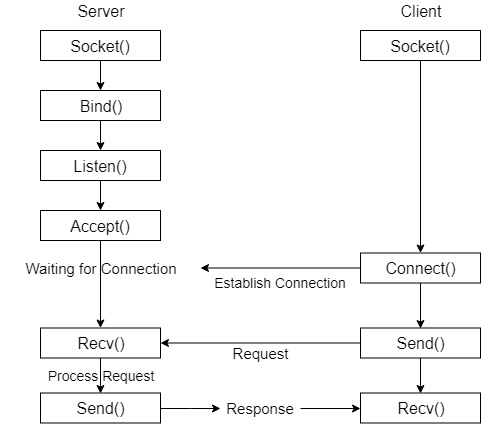
\includegraphics[scale=0.5]{client_server/images/socket.jpg}
\caption{Socket Diagram}
\label{fig:socket}
\end{figure}

The sender and receiver threads achieve data synchronization using event and queue. When the client sends a request message to the server, server returns a message queue while the client is waiting for it. Whenever this event is set, data in queue  will be available to the client. This synchronization process is shown in Figure 5.2.

\begin{figure}[h!]
\centering
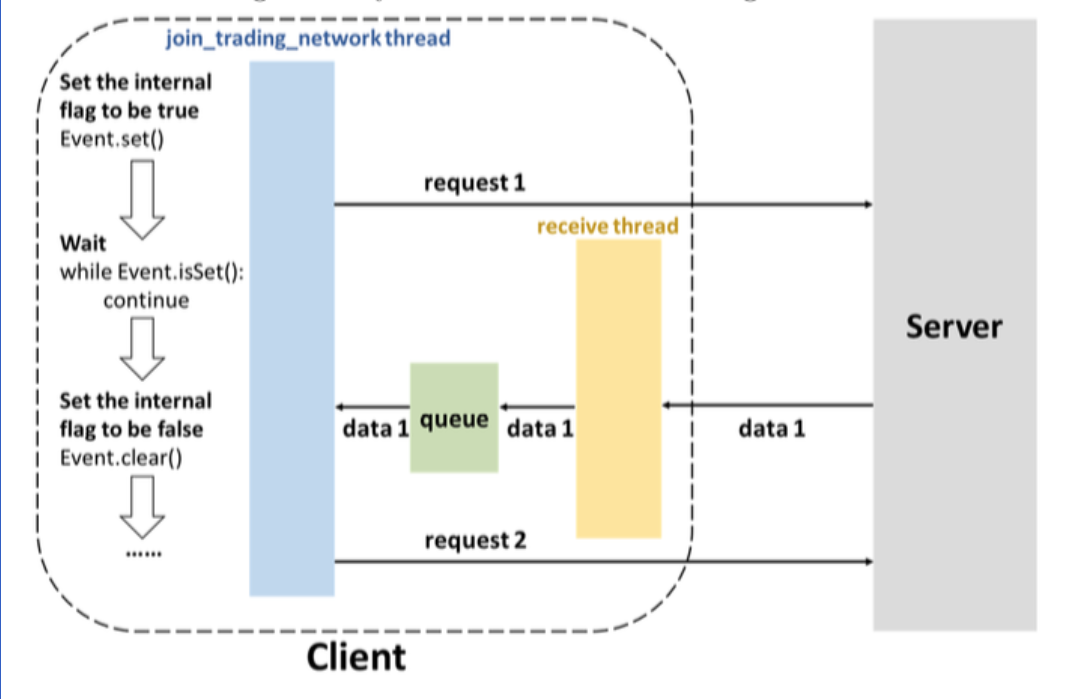
\includegraphics[scale=0.5]{client_server/images/event.png}
\caption{Synchronization Process Diagram}
\label{fig:synch}
\end{figure}


\section{Order Book}
    
Server will provide consolidated books for 30 trading days: 
\begin{enumerate}
    \item Simulated from market data starting from 1/2/2019.
    \item Order book is consist of: order index, symbol, side (buy or sell), price, quantity, and order status, shown in Figure 5.3.
    \item Each simulated trading date has one new book for every 30 seconds from daily historical data, with buy orders and sell orders simulated from the high and low price from the day, with price step of 0.05 and daily volume randomly distributed cross all price points. 
    \item Each simulated trading day lasts 30 seconds, following by 5 seconds of pending closing phase and 5 seconds of market closed phase before market reopen. There are 5 phases of market: 
    \begin{enumerate}
        \item Not Open, start of simulated trading
        \item Pending Open, 
        \item Open, 30s
        \item Pending Close, 5s
        \item Market Close, 5s
    \end{enumerate}
    \item The book supports partial fill, based on comparison of order quantity and available quantity on the book. The order status could be New, Filled or Partial Filled.
    \item If the market status is pending close, trade price will be worse by 0.01.
    \item All orders placed are limit orders.
\end{enumerate}

\begin{figure}[h!]
\centering
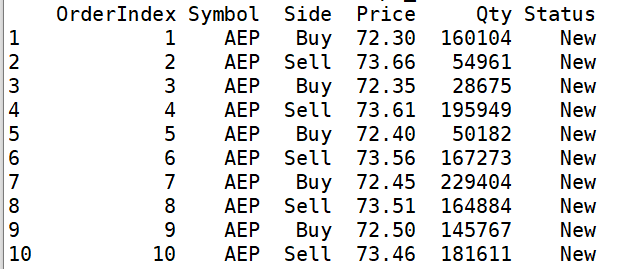
\includegraphics[scale=0.8]{client_server/images/orderbook.png}
\caption{Order Book}
\label{fig:order}
\end{figure}
